\documentclass[conference]{IEEEtran}
%\IEEEoverridecommandlockouts
% The preceding line is only needed to identify funding in the first footnote. If that is unneeded, please comment it out.
\usepackage[spanish]{babel}
\usepackage[utf8]{inputenc}
\usepackage{cite}
\usepackage{amsmath, amsthm,amssymb,amsfonts}
\usepackage{algorithmic}
\usepackage{graphicx}
\usepackage{textcomp}
\usepackage{xcolor}
\def\BibTeX{{\rm B\kern-.05em{\sc i\kern-.025em b}\kern-.08em
    T\kern-.1667em\lower.7ex\hbox{E}\kern-.125emX}}

% Definición del entorno 'definition'
\newtheorem{definition}{Definición}

\begin{document}

\title{Control de sistemas dinámicos mediante operadores fraccionarios: Retos y aplicaciones\\
	% {\footnotesize \textsuperscript{*}Note: Sub-titles are not captured in Xplore and
	% should not be used}
	% \thanks{Identify applicable funding agency here. If none, delete this.}
}

\author{
	\IEEEauthorblockN{1\textsuperscript{st} José Alejandro León Sánchez}
	\IEEEauthorblockA{\textit{Posgrado de Ingeniería} \\
		\textit{UNAM}\\
		CDMX, Mexico}
	\and
	\IEEEauthorblockN{2\textsuperscript{nd} Dr. Marcos Ángel González Olvera}
	\IEEEauthorblockA{\textit{UACM} \\
		CDMX, Mexico}
}

\maketitle

\begin{abstract}
	Este documento es un resumen de la primera ponencia del Seminario de Investigación de la Maestría en Ingeniería Eléctrica (Especializacíon de Control) del programa de Posgrado en Ingeniería de la UNAM. La cual fue presentada por el Dr. Marcos Ángel González Olvera. En esta presentacíon se abordó el uso del cálculo fraccionario en el control de sistemas dinámicos, analizando aplicaciones y desafíos. Se discutieron los retos y ventajas que ofrece esta metodología para el modelado y control de sistemas y se presentaron aplicaciones de diversas áreas, desde ingeniería biomédica hasta robótica.
\end{abstract}

\begin{IEEEkeywords}
	Control de sistemas, operadores fraccionarios, sistemas dinámicos.
\end{IEEEkeywords}

\section{Introducción}
En los últimos años, el interés de la comunidad científica por el uso de operadores fraccionarios en problemas de modelado, control, observación e identificación de sistemas dinámicos ha crecido considerablemente. El cálculo fraccionario, aunque históricamente se remonta a los trabajos pioneros de Leibniz, Euler, y Laplace, ha ganado nueva relevancia en la investigación contemporánea, impulsado por contribuciones más recientes de Bode, Riemann, Liouville, Caputo, entre otros. Esta rama de la matemática no solo presenta desafíos abiertos, como la definición precisa de operadores y el desarrollo de métodos numéricos eficientes, sino que también ofrece un amplio campo de estudio con aplicaciones prometedoras en ingeniería de control, lo que subraya su importancia emergente en el panorama científico actual.
\section{Definición de operadores fraccionarios}
El cálculo fraccionario generaliza el cálculo diferencial e integral clásico, extendiendo la noción de derivada e integral a potencias fraccionarias.

\subsection*{Operadores enteros}
Comúnmente, definimos al operador derivada de la siguiente forma:
Dada una función $f(t), f: \mathbb{R} \rightarrow \mathbb{R}$, el operador derivada $D$ para orden $1$ se define como
\begin{equation}
	D\{f(t)\} := Df(t) = \lim_{\Delta t \rightarrow 0} \frac{f(t + \Delta t) - f(t)}{\Delta t},
\end{equation}
de forma recursiva, para orden $n, n \in \mathbb{N}$ se define como
\begin{equation}
	D^2 f(t) = D^{1}\{D^1f(t)\}, \dots , D^n f(t) = D\{D^{n-1}f(t)\}.
\end{equation}

De manera análoga, el operador integral $I$ se define como:
\begin{equation}
	I^1 f(t) = \int_{0}^{t} f(\tau) d\tau
\end{equation}
y de forma recursiva para orden $n, n \in \mathbb{N}$ se define a través de la conocida integral múltiple de Cauchy:
\begin{equation}
	\begin{aligned}
		I^n f(t) & = \int_{a}^{t} \int_{a}^{\tau_1} \dots \int_{a}^{\tau_{n-1}} f(\tau) d\tau \dots d\tau_2 d\tau_1 \\
		         & = \frac{1}{(n-1)!} \int_{a}^{t} (t - \tau)^{n-1} f(\tau) d\tau.
	\end{aligned}
\end{equation}
\subsection*{Contribución de Euler}
Se sabe que la derivada de una función polinomial $f(x) = x^m$ es:
\begin{equation}
    D_x^n\{ f(x) \} = \frac{m!}{(m-n)!} x^{m-n},
\end{equation}
si $m$ es no entero, Euler propone usar la función gamma $\Gamma(z)$ (Fig. \ref{fig:gamma} ) como sustituta de la función factorial
\begin{equation}
    \Gamma(z+1) = \int_{0}^{\infty} t^{z-1} e^{-t} dt = (z-1)\Gamma(z-1)
\end{equation}
\begin{figure}[h]
    \centering
    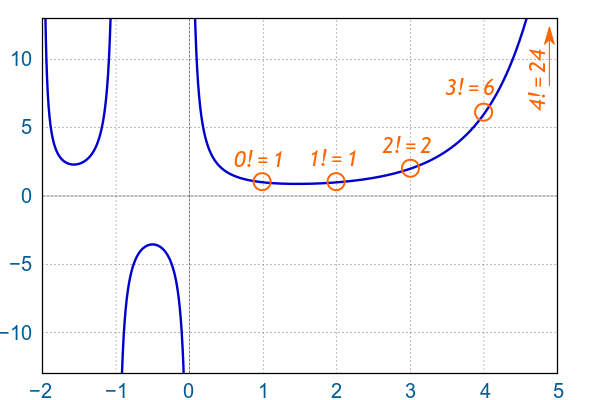
\includegraphics[width=0.5\textwidth]{gamma-plot.png}
    \caption{Función gamma}
    \label{fig:gamma}
\end{figure}
Esto presenta una forma de derivar de forma \textit{no entera} a una función polinomial, es decir, cualquier función que pueda ser expresada por una expansión polinomial se puede derivar de forma fraccionaria.

Retomando la integral múltiple de Cauchy, y con la idea de Euler para sustituir el factorial, se puede definir la integral fraccionaria de Riemann-Liouville como:
\begin{equation}
    I^{\alpha} f(t) = \frac{1}{\Gamma(\alpha)} \int_{a}^{t} (t - \tau)^{\alpha - 1} f(\tau) d\tau,
\end{equation}
con $\alpha \in \mathbb{R}, \mathbb{C}$.

A partir de esto, se han tomado diferentes definiciones para el operador derivada fraccionaria, siendo las más comunes las de Riemann-Liouville\cite{riemann} y Caputo\cite{caputo}:
\begin{equation}
    D^{\alpha} f(t) = \frac{1}{\Gamma(n-\alpha)} \frac{d^n}{dt^n} \int_{a}^{t} \frac{f(\tau)}{(t - \tau)^{\alpha-n+1}}  d\tau, \quad \alpha \in (n-1, n)
\end{equation}
\begin{equation}
    D^{\alpha} f(t) = \frac{1}{\Gamma(n-\alpha)} \int_{a}^{t}  \frac{\frac{d^n}{dt^n} f(\tau)}{(t - \tau)^{\alpha-n+1}} d\tau, \quad \alpha \in (n-1, n)
\end{equation}

Algunas propiedades interesantes de estas definiciones son:
\begin{itemize}
    \item Con la derivada fraccionaria de Caputo se puede interpretar físicamente la condición inicial.
    \item Con la derivida fraccionaria de Riemann-Liouville se limitan las aplicaciones por la auscencia de interpretación física de los valores límite en $t=0$.
    \item En problemas donde $f(t) = 0 \forall t \leq 0$ ambas soluciones convergen.
\end{itemize}

\section{Aplicaciones}\label{AA}
Algunos ejemplos de sistemas físicos con modelos de orden fraccionario son:
\begin{itemize}
    \item Lineas de transmisión semi-infinitas.
    \item Fenómenos difusivos.
    \item Modelos opidemiológicos.
    \item Oscilaodres no caóticos.
    \item Mecánica y dinámica de fluidos.
    \item Fenómenos viscoelásticos en materiales biológicos.
    \item Coordinación de múltiples robots.
\end{itemize}

Una de las aplicaciones sencillas y destacadas es el control PID fraccionario (Fig. \ref{fig:frac-pid}) que, a pesar de ser un controlador simple, presenta un comportamiento más robusto que el controlador PID clásico, con otras ventajas como la reducción de problemas de saturación cuando se \textit{deriva menos}. En general, este controlador vuelve más lenta la respuesta del sistema, pero menos sucetible a ruido y perturbaciones.

\begin{figure}[h]
    \centering
    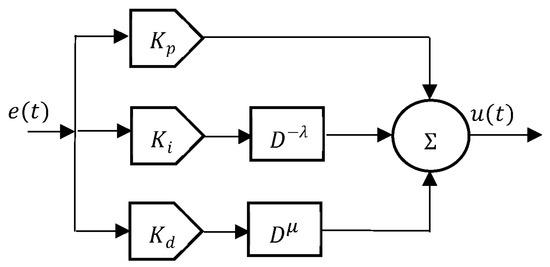
\includegraphics[width=0.5\textwidth]{fractional-pid.jpg}
    \caption{Control PID fraccionario}
    \label{fig:frac-pid}
\end{figure}

\section*{Conclusiones}
El uso de operadores fraccionarios en el control de sistemas dinámicos ha demostrado ser una herramienta poderosa y versátil, especialmente en situaciones donde los modelos convencionales de orden entero no capturan adecuadamente la dinámica del sistema. A través de este estudio, se ha observado que los operadores fraccionarios permiten una mayor flexibilidad en el modelado y control, lo que conduce a sistemas con respuestas más robustas y menos sensibles a perturbaciones.

El control PID fraccionario, como se discutió, es un ejemplo claro de cómo la implementación de cálculo fraccionario en sistemas de control puede mejorar significativamente el rendimiento del sistema. 

Sin embargo, aún existen desafíos en la implementación práctica de estos métodos, como la necesidad de desarrollar algoritmos numéricos más eficientes y comprender mejor las implicaciones físicas de los operadores fraccionarios. A pesar de estos retos, las aplicaciones potenciales de este enfoque, desde la ingeniería biomédica hasta la robótica, indican que el cálculo fraccionario continuará siendo un área de investigación activa y en crecimiento en los próximos años.

\begin{thebibliography}{00}
	\bibitem{caputo} M. Caputo, ``Linear models of dissipation whose Q is almost frequency independent—II,'' \textit{Geophysical Journal International}, vol. 13, no. 5, pp. 529--539, 1967.
	
	\bibitem{riemann} J. Liouville, ``Mémoire sur quelques questions de géométrie et de mécanique, et sur un nouveau genre de calcul pour résoudre ces questions,'' \textit{Journal de l'École Polytechnique}, vol. 13, no. 21, pp. 1--69, 1832.
\end{thebibliography}

\end{document}
